\chapter{protocol}
	
	The commitment tree is a tree where each vertex has an associated label representing the data that is passed on to its parent. The messages have the following format: 
	\textit{MESSAGE}
	\newline
	
	\begin{tabular}{ | l | l | l | l |}
		\hline
		ID & COUNT & VALUE & COMMITMENT \\
		\hline
		20 bits & 21 bits & 20 bits & 256 bits\\
		\hline
	\end{tabular}
	\newline
	\newline
	\textit{SIGNATURE (MESSAGE)}
	\newline

	\begin{tabular}{ |l| }
		\hline
		Encryption$_{secret-key_{node}}$( HASH ( MESSAGE ) )\\
		\hline
		500 bits\\
		\hline
	\end{tabular}
	\newline
	\newline
	\textit{CERTIFICATES}
	\newline

	\begin{tabular}{ | l | l | l | }
		\hline
			Public key  & Signature & ID \\
		\hline
			1000 bits & 500 bits & 20 bits \\
		\hline

	\end{tabular}

	\newpage

\section{Aggregation-Commit Phase}
	In this phase, the sensor nodes construct a commitment forest. 
	First, the sensor nodes at the highest depth in the aggregation tree (leaf nodes) send their messages to their parents in the aggregation tree.
	Each internal sensor node in the aggregation tree performs an aggregation operation whenever it receives messages from all of its children.
	Whenever a sensor node performs an aggregation operation, it creates a commitment to the set of inputs used to compute the aggregate by computing a hash over all the inputs (including the commitments that were computed by its children). 
	Both the aggregation result and the commitment creates a message.
	Then the message, with the signature of the message signed by the sensor node are passed on to the parent of the sensor node.
	Once the final messages and the signatures of those messages are sent to the querier, if the adversary tries to claim a different aggregation structure it gets caught.
	Our algorithm generates perfectly balanced binary trees to create commitment forest which saves the bandwidth in the verification phase.


	\begin{definition}
		A \textbf{\textit{commitment tree}} is a logical tree build on top of an \textbf{\textit{aggregation tree}} in which each vertex has an associated message to it, representing data being passed on to its parent. The messages have the following format:\\

		$<id, count, value, commmitment>$\\
		\newline
		Where $id$ is the unique id of each vertex; $count$ is the number of leaf vertices in the subtree rooted at this vertex; $value$ is the aggregate computed over all the leaves rooted in the subtree; and commitment is the cryptographic commitment.

	\end{definition}

	There is one leaf vertex $v_{s}$ for each sensor node $s$ with the message $m_{s}$ = $< s.id, 1,s.value, Hash( N\ ||\  s.id\ ||\  1\  ||\  s.value) > $, where N is the query nounce.

	Internal vertices represent aggregation operations, and have messages that are defined based on their children. Suppose an internal vertex has child vertices $v_{1}, v_{2},\dotsc, v_{q}$ with the following messages: $m_{1}, m_{2},\dotsc, m_{q}$, where $m_{i}$ = $<i.id$, $i.count$, $i.value$, $i.commitment>$.
	Then the vertex has message $<id, count, value, commitment>$ where $id = s.id$, $count = \sum{i.count}$, $value = \sum{i.value}$ and $commitment$ = $H[$ $N\ || $ $id\ || $ $count\ || $ $value\ ||$ $m_{1}\ ||\ m_{2}\ || \dotsb ||\ m_{q}]$.

	Since we use the hash function which is collision resistant its impossible for an adversary to change the any of the commitments.

	\textit{\textbf{Write about off-path values also about forests }}

	\begin{figure}[hp]
		\centering
		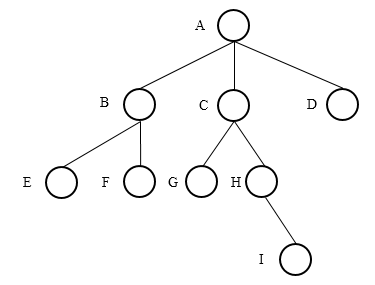
\includegraphics[scale=0.8]{images/featured-tree.png}\\
		\caption{Fetured Tree}
	\end{figure}

	\textit{\textbf{Output forest for given sensor node using binary representaion}}

	Binary representation of number of descendants for a given sensor node tells us about the structure of that sensor node's output forest. 
	It tells us the number of binary trees with their respective heights for given sensor node's output forest.
	For example, if sensor node $A$ has $8$ descendants then $A$ has to aggregate $9$ messages including itself during aggregation process.
	And we can write the following:	$(9)_{10}$ = $(1001)_{2}$ 
	It means $A$ has two binary trees in its output forest, one with height of three and one with height of one.

	\textit{\textbf{ Aggregation using binary representation}}

	\[ 
		\begin{array}{lcccc}
			\mbox{Carry} & 0 & 1 & 1 & 0\\
			\hline
			\mbox{Trees in B's forest} & 0 & 0 & 0 & 1 \\
			\mbox{ } & 0 & 0 & 1 & 0 \\
			\hline
			\mbox{Tree in C's forest} & 0 & 1 & 0 & 0 \\
			\hline
			\mbox{Tree in D's forest} & 0 & 0 & 0 & 1 \\
			\hline
			\mbox{A's own message} & 0 & 0 & 0 & 1 \\
			\hline
			\mbox{Aggregation} & 1 & 0 & 0 & 1 
		\end{array}
	\] 

\newpage
\begin{algorithm}[H]\label{number3} \caption {CommitmentTreeGeneration}
	\begin {algorithmic}[1]

		\STATE depth = \at.MaxDepth
		\WHILE {depth $\geq$ 0}

			\FORALL {\node \   $\in$ \at.depth }

			\STATE \node.\forest = NULL
					\STATE Create (\node.\msg, \sign $_{\cal{N}}$(\node.\msg))
					\STATE Attach (\node.\msg, \sign $_{\cal{N}}$(\node.\msg)) to \node.\forest
					
					\IF {\node.\children \ $\neq$ \ 0}

						\FORALL {\child \ $\in$ \node.\children }

							\FORALL {tree root \treeRoot \ $\in$ \child.\forest}

								\IF {\node \ has \treeRoot.\cert (else get \treeRoot.\cert )} 

									\IF {\node verifies \treeRoot.msg (else raise an alarm)}

										\STATE Add \treeRoot \ to \node.\forest
										
									\ENDIF
								
								\ENDIF

							\ENDFOR

							\STATE \node.\forest \ =	CommitmentTreeCoding ( \node.\forest \ ) 
						
						\ENDFOR
		
					\ENDIF


			\ENDFOR

			\STATE {depth = depth - 1 }

		\ENDWHILE
	\end{algorithmic}

\end{algorithm}

\begin{algorithm}[H]\caption{CommitmentTreeCoding}
	\begin{algorithmic}[1]

		\STATE \temp \ = SortLinkedList( \node.\forest \ )

		\WHILE {\temp.\nextTree \ $\neq$ \ 0}

			\IF {\temp.\height \ $\neq$ \ \temp.\nextTree.\height } 
				\STATE \temp \ = \temp.\nextTree
			\ELSE

				\STATE Create an aggregation node \aggregator 
				\STATE \aggregator.\height \ = \temp.\height \ + 1
				\STATE \aggregator.\lc \ = \temp
				\STATE \aggregator.\rc \ = \temp.\nextTree
				\STATE Insert \aggregator \ to \node.\forest
				\STATE Remove \temp
				\STATE Remove \temp.\nextTree
				\STATE \temp \ = SortLinkedList( \node.\forest \ )

			\ENDIF

		\ENDWHILE		

		\STATE return \temp

	\end{algorithmic}

\end{algorithm}

\newpage

\begin{algorithm}
\caption{Pseudo algorithm to detect a cheater}

	\begin{algorithmic}[1]

			\STATE \querier \ finds out all the \complainer$_{\mathcal{N}}$ $\in$ \at \ using a complainer detecting algorithm

			\FORALL {\complainer$_{\mathcal{N}}$}

				\STATE \querier \ gets \node$_{0}$, \sign $_{\cal{N}}$ ( \node$_{0}$ )
			
			\ENDFOR

			\STATE \querier \  finds possible \cheater \ based on \complainer$_{\mathcal{N}}$

			\FORALL {\cheater}

				\STATE \querier \  gets \node$_{\mathcal{I}}$, \sign $_{\cal{N}}$ ( \node$_{I}$ ) \cheater \  receives and sends. 
				\STATE If needed \querier \  gets \node$_{\mathcal{I}}$, \sign $_{\cal{N}}$ ( \node$_{I}$ ) of the \parent \ \cheater 
			
			\ENDFOR

			\STATE \querier \  determines the \cheater \ based on recived information

	\end{algorithmic}
\end{algorithm}

\textit{Properties of commitment tree and aggregation tree}

	If you have $O(n)$ children then you need atleast $\Omega(n)$ \& at max $O(nlog(n))$ certificates.

	If you have $O(n)$ descendents then you need $\Omega(log(n))$  \& at max $O(nlog(n))$ certificates.
